    \section{Motivation and mathematics for feedforward}
    \label{motive_math}

LIGO, the Laser Interferometer Gravitational-wave Observatory [Hanford, Washington and Livingston, Louisiana] measures the differential length of 4-km Michelson arms with Fabry-Perot cavities. Length changes could indicate strain caused by astrophysical sources of gravitational waves. Fundamentally limited by seismic noise, thermal suspension noise, and laser shot noise in different frequency bands, a LIGO interferometer's sensitivity can also be degraded by additional relative motion of the inner arm cavity mirrors due to imperfectly-servoed Michelson motion. In this project we seek to subtract the effects of this residual motion by feedforward correction of the gravitational-wave data channel. We divide data from LIGO's sixth science run into 1024-second time windows and numerically fit a filter representing the frequency-domain transfer function from Michelson servo noise to gravitational wave channel for each window. Finally, the Michelson servo channel is processed through the filter and is subtracted from the gravitational-wave signal channel. The algorithm used in this procedure will be described with a preliminary assessment of the achievable sensitivity improvement.

        Before delving into the details of the algorithm, a primer on the motivation and mathematics should follow. LIGO and its predecessors have long relied on servo control using feedforward and feedback to stabilize interferometers. At the 40 meter interferometer at Caltech, an early experiment to subtract noise post-facto was attempted (Bruce Allen? Find earliest citation -- Keith or Rana would know). Yet most schemes in the modern era have relied on realtime methods. Fundamental noise sources would be unapproachable if we did not.

        LIGO by design should be limited only by fundamental, physical sources of noise. Initial and Enhanced LIGO are bound at low frequencies by seismic noise, at its middle and most sensitive frequencies by thermal noise from its suspensions, and at its highest frequencies by laser shot noise. Advanced LIGO, if commissioning succeeds, will be purely quantum mechanically limited: radiation pressure will dominate the low frequencies and shot noise the high. These sources can only be ameliorated with better hardware. Yet we have reason to suspect that the real instruments are not so perfect: some noise remains that is both caused by and can be fixed by better software -- in particular, better servos.  

        Myriad LIGO systems are servoed, from laser frequency to mirror position. The entire aim of these servos is to provide a more sensitive measurement of differential arm motion, which directly corresponds to \textit{h(t)}, the gravitational wave signal. Some servos affect \textit{h(t)} more directly than others. The differential arm motion of the outer mirrors is itself refered to as $DARM$, and the three other motions of the mirrors have a special importance as well: $CARM$, the common outer arm motion, $MICH$, the differential "Michelson" motion of the inner mirrors, and $PRC$, the "power recycling cavity" common motion of the inner mirrors.   

The four LIGO mirror test masses (TM) are named by arm (X or Y) and inner (I) vs end (E) of the Fabry-Perot cavities. LIGO controls four length degrees of freedom.

        $$
        \textit{CARM} = L_{+} = \frac{L_y + L_x}{2},
        $$
        $$
        \textit{DARM} = L_{-} = L_y - L_x,
        $$
        $$
        \textit{PRC} = l_{+} = \frac{l_y + l_x}{2},
        $$
        $$
        \textit{MICH} = l_y = l_y - l_x,
        $$

        $$
        L_y \equiv d(\textit{ETMY} - \textit{ITMY}),
        $$
        $$
        L_x \equiv d(\textit{ETMX} - \textit{ITMX}),
        $$
        $$
        l_y \equiv d(\textit{ITMY} - \textit{RM}),
        $$
        $$
        l_x \equiv d(\textit{ITMX} - \textit{RM}).
        $$

\begin{figure}
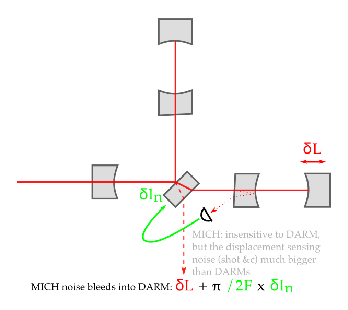
\includegraphics[height=90mm,width=160mm]{ligo_michdamp.eps}
\caption{MICH noise seen as DARM/(arm gain); PRC too seen in DARM}
\label{arms}
\end{figure}

        In initial LIGO, for historical interest, but not precisely so in enhanced or advanced LIGO,

        $$
        \aleph \equiv 4 J_0 (\Gamma) J_1 (\Gamma) P \cos \omega_m t,
        $$
        $$
        [L_{-} \rightarrow \textit{AS}_Q] = -\aleph g_{cr}t_sb r_c ' \frac{1}{1 + if/f_c} k \delta L_{-},
        $$
        $$
        [l_{-} \rightarrow \textit{AS}_Q] = \aleph g_{cr} t_{sb} r_c \frac{1}{1+if/f_c} k \delta l_{-}.
        $$

        %\begin{figure}[htb]
        %\begin{center]
        %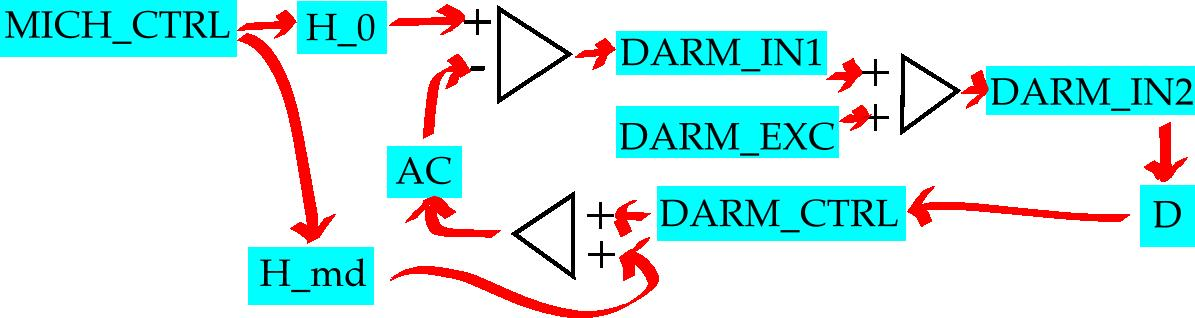
\includegraphics[width = 0.45\paperwidth, keepaspectratio]{servo_loop.jpg}
        %\caption{Servo loop}
        %\label{Servo loop}
        %\end{center}
        %\end{figure}

        Conclusion about MICH-DARM coupling: Noisy MICH resembles DARM \textit{sans} arm gain.

        $$
        r_{c}' = \pi / (2F) \approx 137 r_c
        $$

        

        \subsection{Auxiliary noise coherence at sensitive frequencies}
        \label{aux_noise}

	    DARM is coherent with MICH and PRC, as can be seen in figures (ADD LABELS), in the most sensitive band for gravitational wave detection. Coherence is the frequency-dependant analog of statistical correlation: on a scale of 0 to 1, it represents the normalized fraction of a frequency bin in the spectrum of one channel that is in a constant phase and amplitude relation with the corresponding frequency bin in the spectrum of another channel. It thus represents the degree of linear coupling between those channels. Channels that have a low value of coherence across their spectrum can be viewed as relatively linearly indepedent of one another. 

        For the coherence between MICH and DARM, values of up to 0.1 were seen in the band of a few hundred Hertz before Keita Kawabe and I implemented the realtime version of our version. The PRC-to-DARM coherence was several times smaller and thus deemed insignificant. When we implemented our filter, the MICH values diminished several-fold (ADD SCREENSHOT?), demonstrating the filter's efficacy.

	In the post-facto work, we had to design a system that could effectively fit a filter in the most-coherent band across many different segments. We surveyed S6 LIGO science segments until focusing on the 80 to 400 Hz (DOUBLE CHECK) band as the most coherent for both MICH and PRC coupling into DARM, or rather, its calibrated counterpart, Hoft. Note that coherence is, ideally, transitive. Since Hoft is simply DARM passed through a linear filter, the coherence between any channel and Hoft should be, to within numerical precision, identical to the coherence between that channel and DARM. We then decided to fit heavily in this region. As referenced by Greg Mendell (cite his 2013 March LVC talk if necessary), the statistical significance of a transfer function -- and thus our measure of the coupling from noise into signal -- is assessed through coherence. By fitting only in regions where the coherence was typically greater than 0.03 (CHECK: is this about the right number?), we verified that the uncertainty in our transfer function was no greater than (CHECK: what is the number?). Outside this band we both deweighted the fit to the transfer function and pre-processed the transfer function, surpressing it by factors of $(f/f_\textup{knee})^\alpha$, where $\alpha$ = 8 at low frequencies and -8 at high. Both the deweighting and the pre-processsing must be carefully-tuned to avoid monopolizing a scarce set of free parameters, the poles and zeros that float to fit the transfer function.

By minimizing the transfer function and thus our fitted filter where it would be incoherent, we avoid adding noise.

        \subsection{Predicted and empirical correction}
        \label{correction}

            Manual, constant correction long applied, known \textit{a priori} cause.

            Draw on Stefan Ballmer/Rana Adhikari and trace down the origin of the MICH and PRC estimates, possibly reiterate with citation. Emphasize that it is frequency-independent, flat, whereas the observed residual coherence is not perfectly flat.

        \subsection{Filter mathematics: in-loop and out-of-loop}
        \label{filter_math}

            Mathematics of in-loop/out-of-loop filtering.

            Discuss servos, including the usual terminology of plants, gain. Principle references: Saulson~\cite{Saulson}, Luca Matone's lectures, possibily some EE texts such as Horowitz and Hill.

	We should also quote Jeff Kissel's thesis~\cite{KisselThesis}, which in chapter 3 has an extensive discussion of DARM, its calibration and response function, the actuation and sensing functions, filters and plants.

        \subsection{Estimating optimal filters}
        \label{filter_est}

            Transfer functions to second-order systems.

		Transfer functions are frequency-domain fit to
		32-pole ZPK (zero-pole-gain) filters, applied in time domain.

            Frequency domain subtraction filtering.

            $$
            T_{xy} (f) = \frac{P_{yx}(f)}{P_{xx}(f)},
            $$
            $$
            P_{yx} (f) = \int_{-\infty}^{+\infty} \left(\int_{-\infty}^{+\infty} y^{*} (\tau) x(t+\tau) d \tau \right) e^{i 2 \pi f t} dt,
            $$
            $$
            g_c(f) = T_{sn} (f),
            $$
            $$
            \hat{s} (f) = (s + g_s \times n)_{m} (f) - g_c (f) \times n_m (f).
            $$

            Where $\hat{s}$ is the post-filter signal, $s$ is the pre-filter signal, $n$ is the noise, $g_s$ is the transfer function coupling noise into signal, $g_c$ is the estimated feedforward filter decoupling noise from signal, and the subscript $m$ indicates an observable or measurable quantity.

\textbf{Sample feedforward from LIGO Hanford Observatory}\\
\textit{2010-03-21T0000Z: MICH on left, PRC on right.}

\begin{figure}
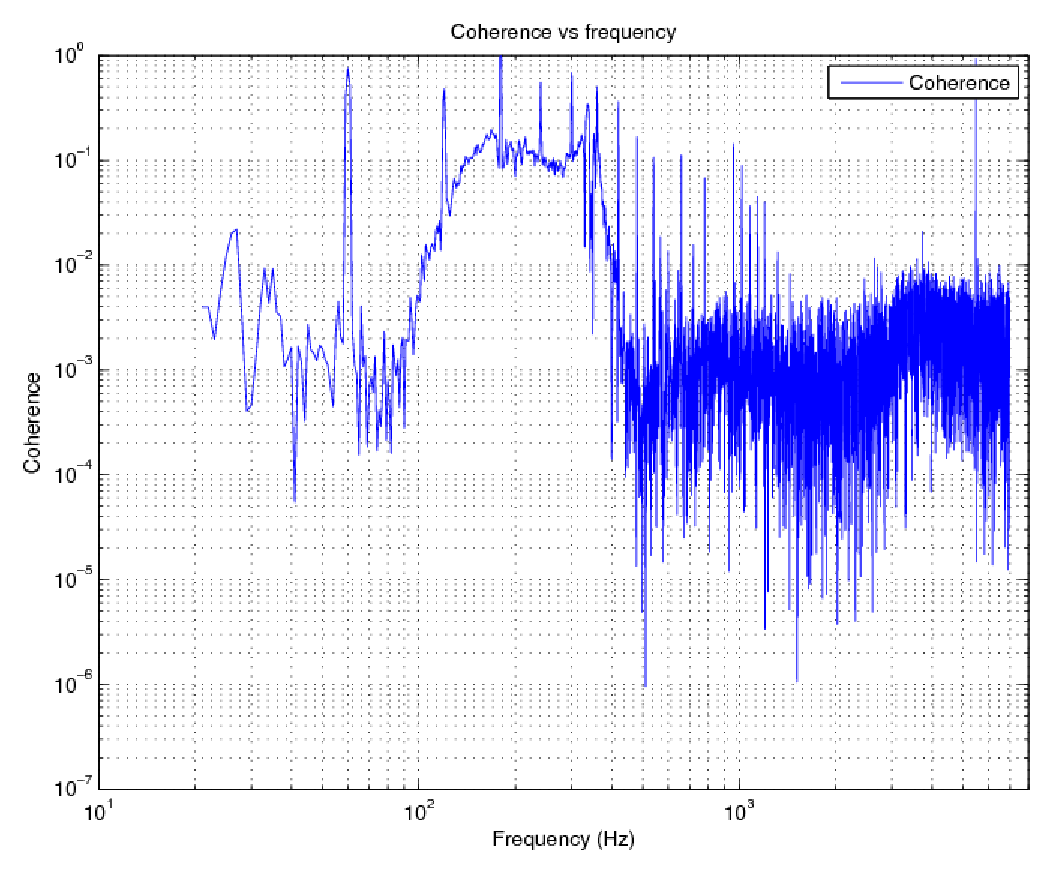
\includegraphics[height=75mm, width=60mm]{clip-MICH-coh.eps}
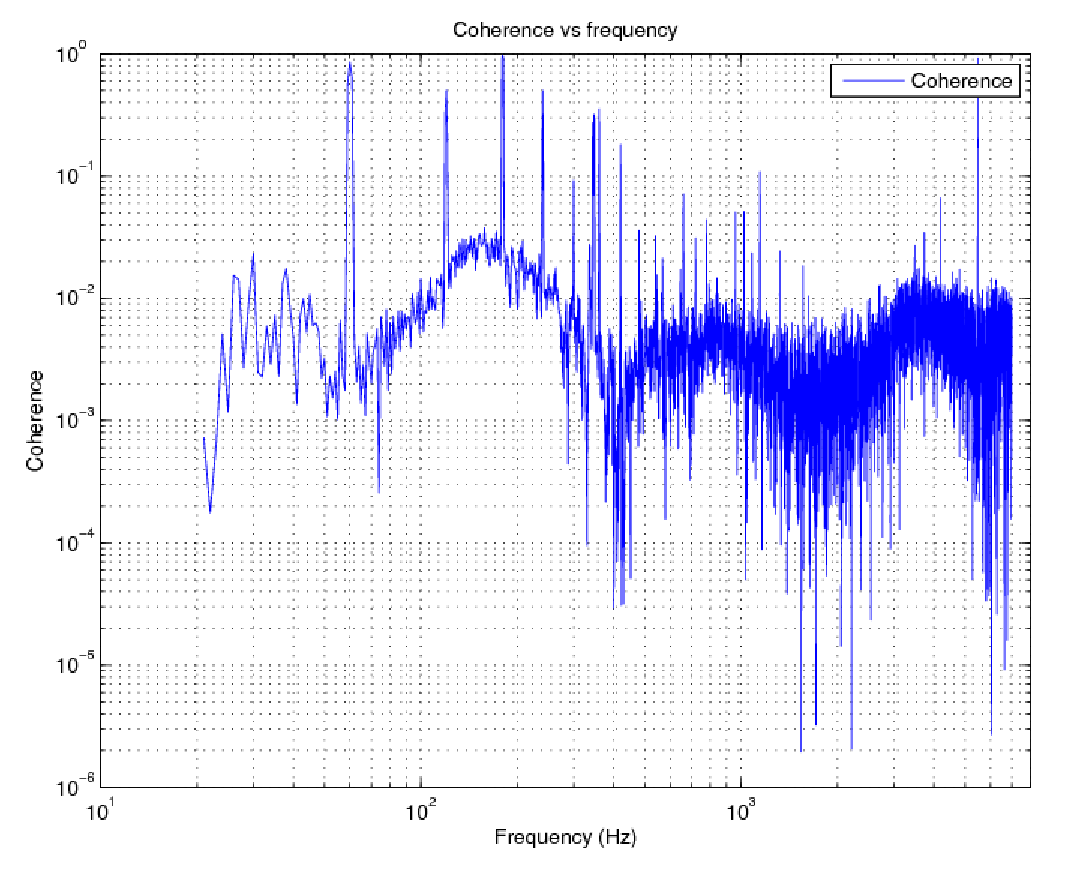
\includegraphics[height=75mm, width=60mm]{clip-PRC-coh.eps}
\caption{Statistically-significant coherence justifies fit}
\end{figure}
\begin{figure}
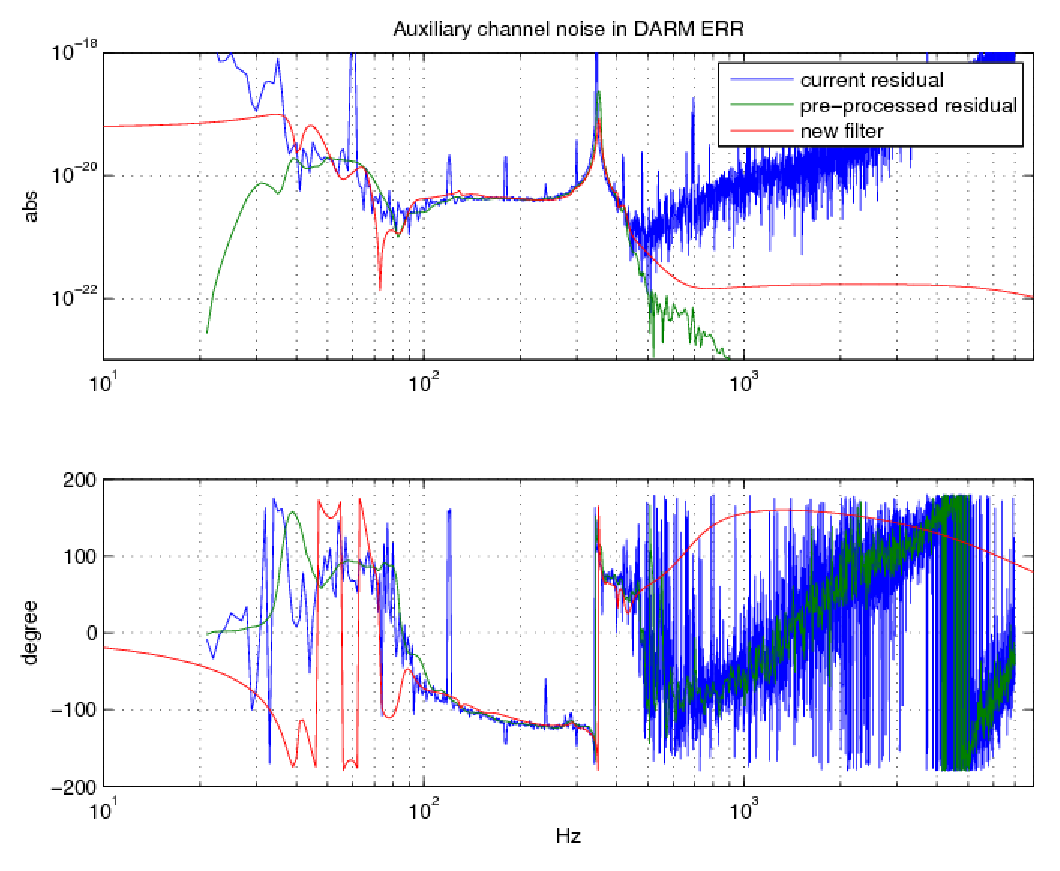
\includegraphics[height=80mm, width=60mm]{clip-MICH-fit.eps}
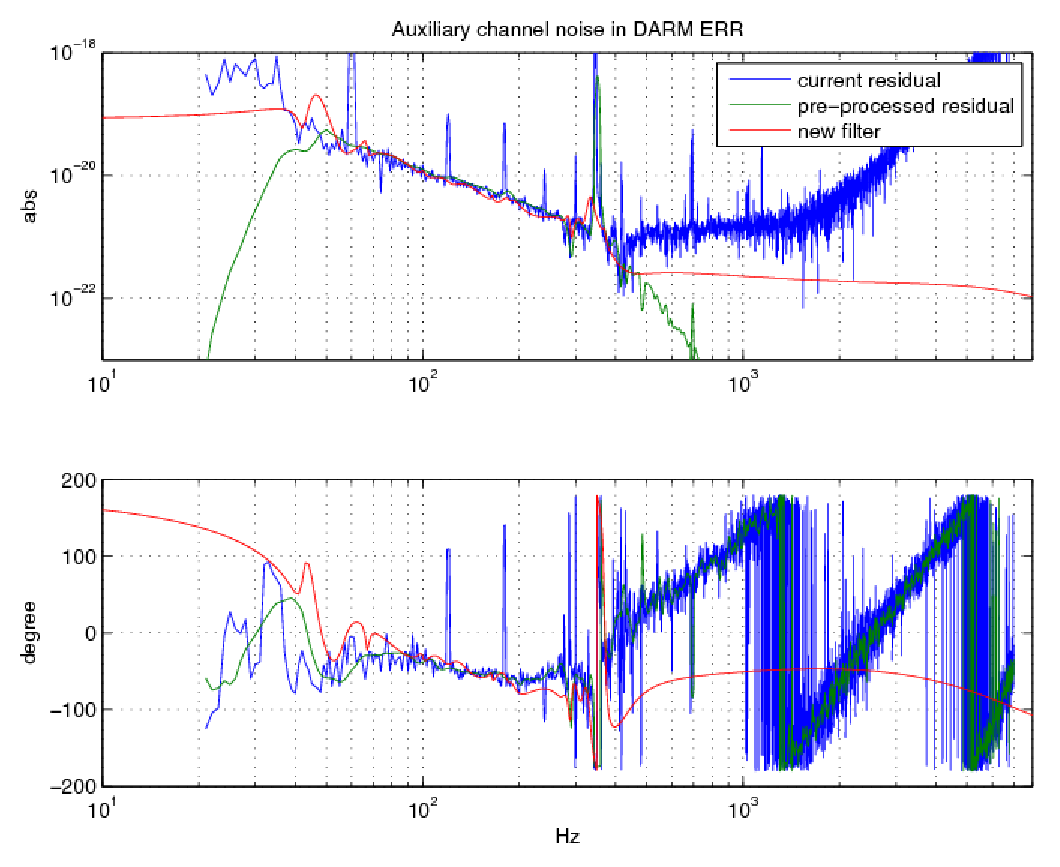
\includegraphics[height=80mm, width=60mm]{clip-PRC-fit.eps}
\caption{Transfer function fit in coherent band}
\end{figure}
\begin{figure}
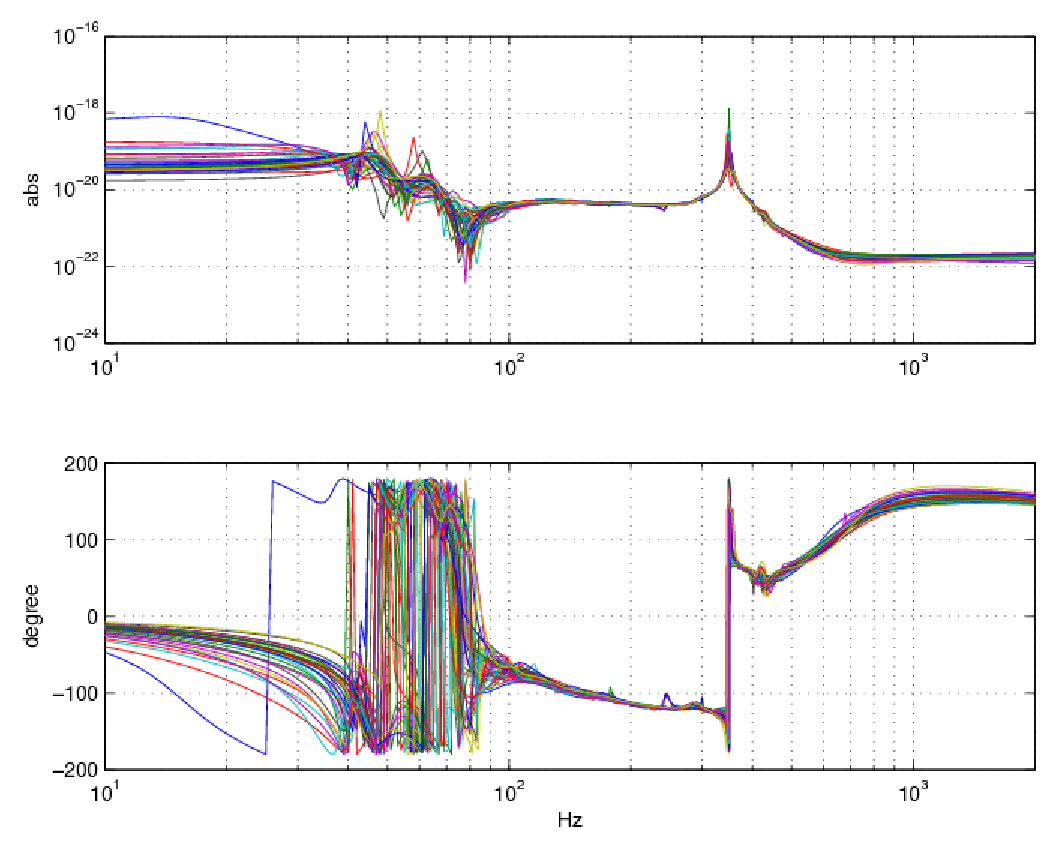
\includegraphics[height=80mm, width=60mm]{clip-MICH-many.eps}
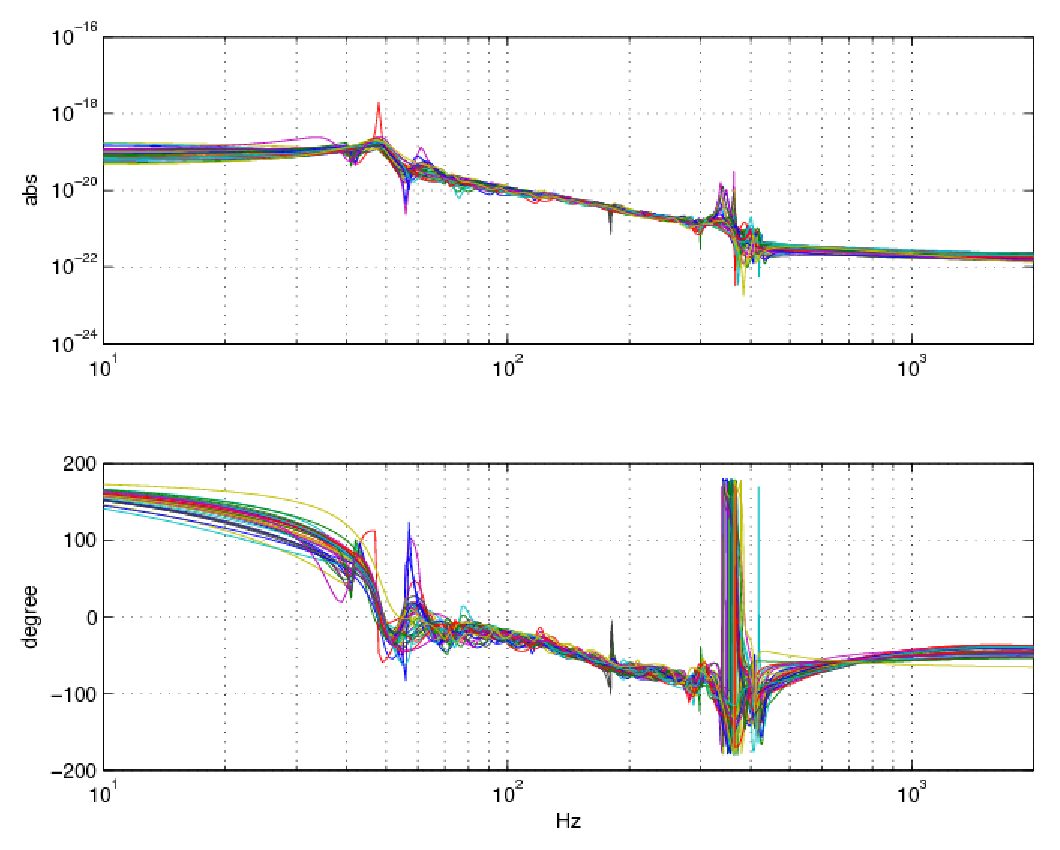
\includegraphics[height=80mm, width=60mm]{clip-PRC-many.eps}
\caption{Fits for 1024 s windows in a science segment}
\end{figure}
\begin{figure}
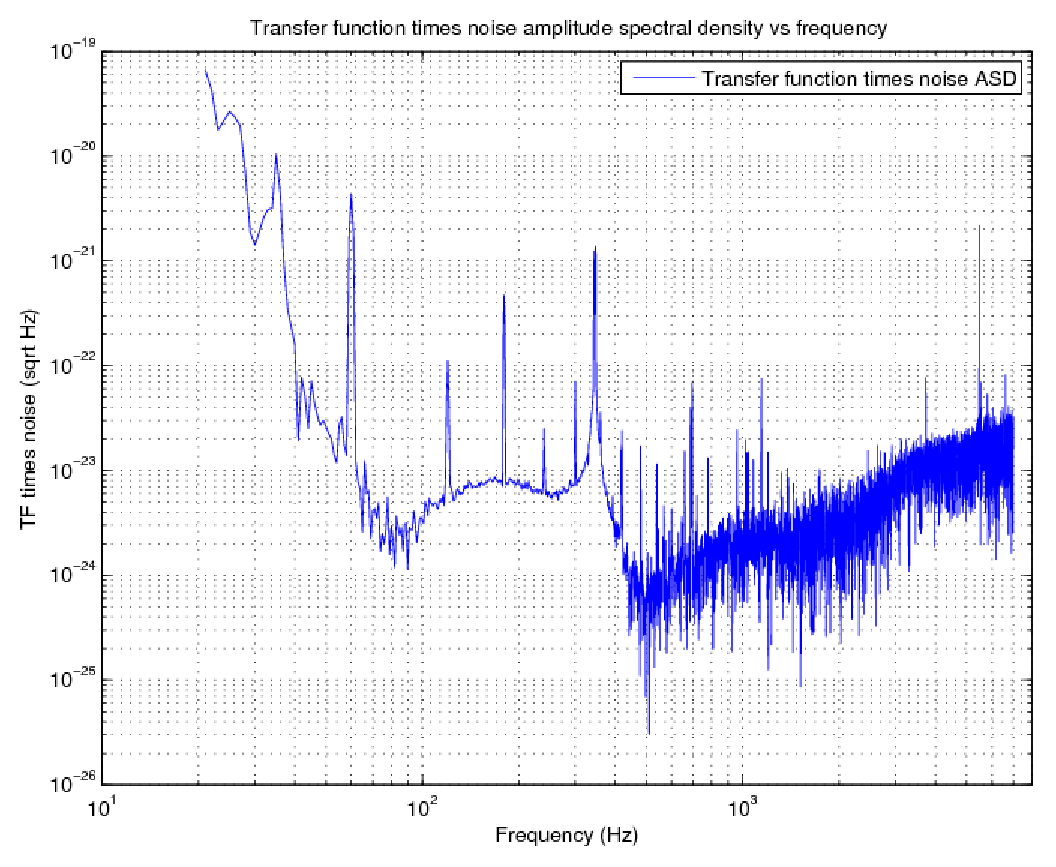
\includegraphics[height=75mm, width=60mm]{clip-MICH-sub.eps}
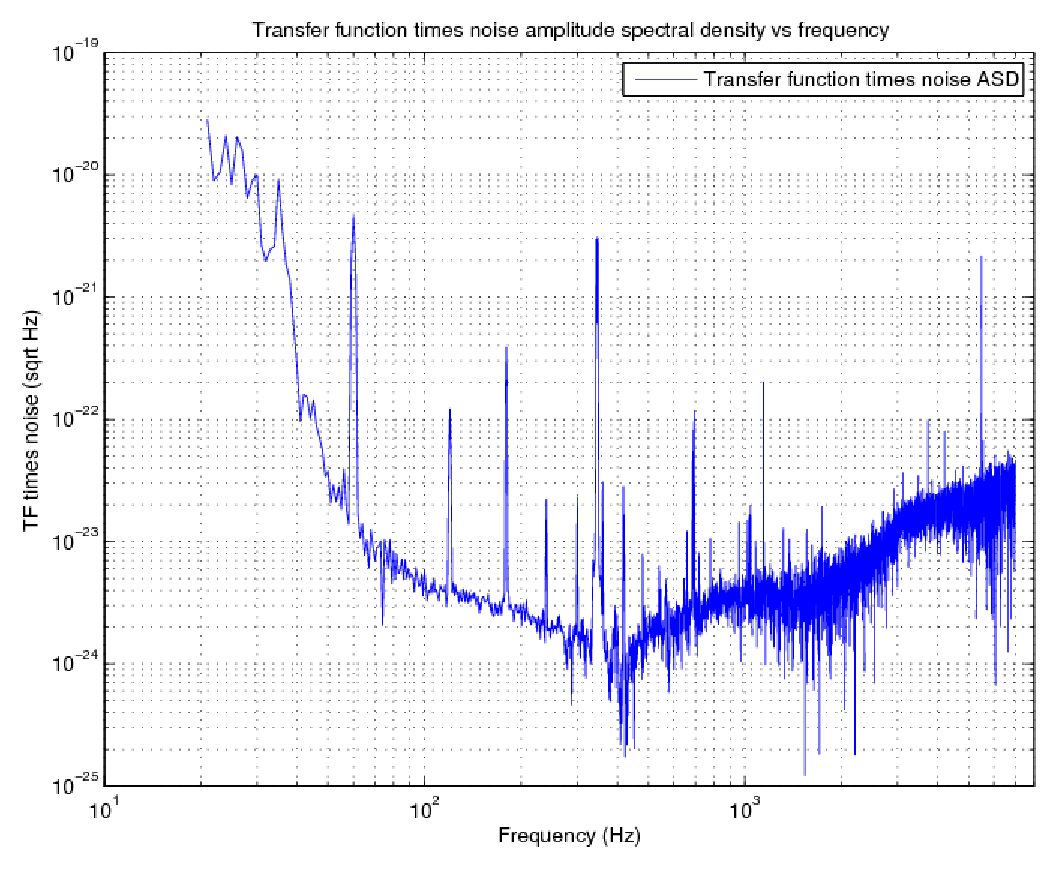
\includegraphics[height=75mm, width=60mm]{clip-PRC-sub.eps}
\caption{Subtracted spectrum for one window}
\end{figure}

    \section{Prior programs}
    \label{prior_programs}
   
        Keita's and Rana's prior programs.
        
        \subsection{Manually-designed rational filtering}
        \label{manual_design}

            Keita's by-hand rational-filter

        \subsection{Vector-fitted filter functions}
        \label{vectfit}

            Rana and Jenne's and Dani's work with vectfit.

        \subsection{Wiener filters}
        \label{wiener_filters}

            Rana and Jenne's 40 m Wiener filtering attempts and why that fails here. Klimenko?

            Wiener filtering searches for an optimal filter of a particular kind: it minimizes the squared error. That error can be the difference between the estimated signal and the time-delayed signal. However, the error is over the entire spectrum. For our problem, we would have to band-pass the spectrum into many sub-spectra, then evaluate the error over those, or else the estimation would be overwhelmed by the power at low-frequencies. The coherence at low-frequencies is low, so basing a filter on those, especially at the expense of higher frequencies, would be unjustified and futile.

    \section{Feedforward in-loop}
    \label{in-loop}

        Feedforward program structure: in-loop.

        \subsection{Filter fitting}
        \label{filter_fitting_in-loop}

            Matlab: obtain frame data, fit, integrate existing filters, export.

        \subsection{Real-time filtering}
        \label{real-time}
      
            Foton: real-time SOS filtering.

    \section{Feedforward out-of-loop}
    \label{out-of-loop}

\begin{figure}
%\includegraphics[height=110mm,bb=25 169 579 609]{jm.fig5.eps}
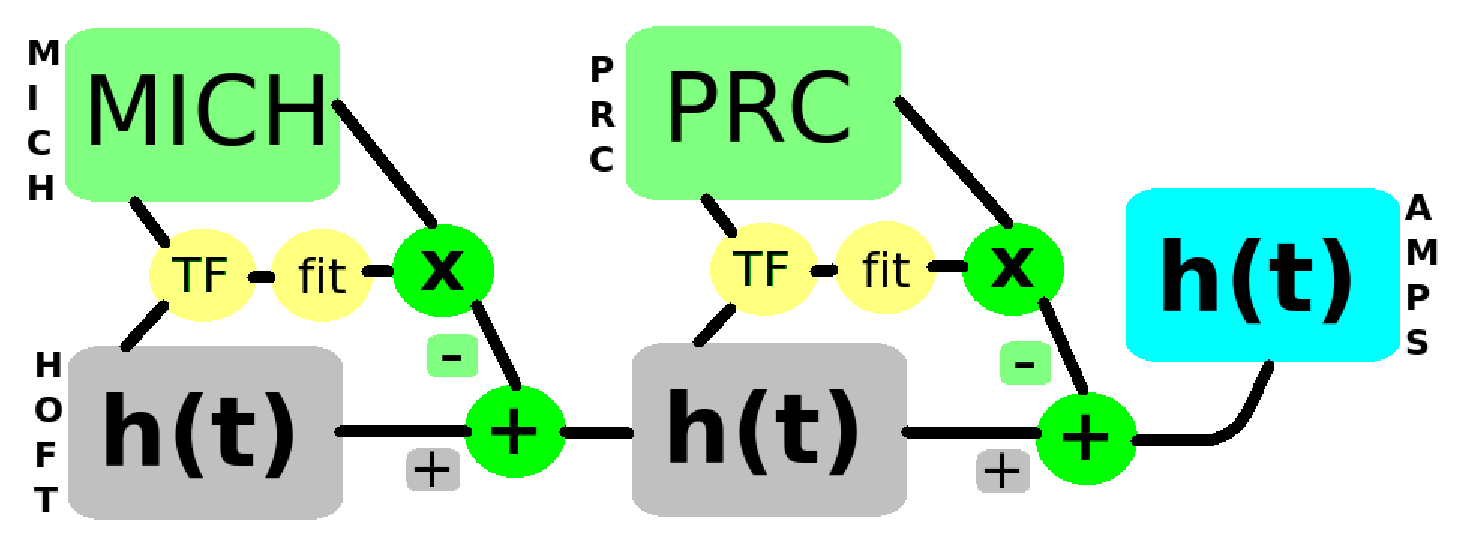
\includegraphics[height=95mm,width=120mm]{pipeline.eps}
\caption{\textit{Feedforward filtering pipeline}}
\label{pipeline}
\end{figure}    
\textup{Read in Hoft (calibrated DARM), MICH, PRC,
write out AMPS (clean calibrated DARM). Code in LIGO SVN:}\\
\texttt{matapps/packages/detchar/} \\ 
\texttt{AMPS/trunk/aletheia.m}
\\


        A critical point: we use the entire set of data for a window to produce a filter, then apply that filter back to the entire set of data. Those familiar with a machine learning view may worry that this is overfitting, that we are not training the data. But that worry really is not justified. The concept of training and over-fitting are valid in the frequency-domain aspect of this work, where we take steps to correct it, such as the pre-processing of the spectrum shape and the post-processing vetos. But in the time-domain, overfit should we restrict the filter-training to a subset of the data? That might make sense if we assumed the data to be stationary and were going to let it run into the future, or if we wanted to learn something scientific about the meaing of the filter coefficients. None of those assumptions hold. We assume the data to be non-stationary, although a complaint could be made that we are unsure about the timescales of non-stationarity. We do not let the filter run arbitrarily into the future, but explicitly window it. Finally, we do not have ambitions to extract scientific meaning from the filter coefficients, although that may change -- even if we did go down that route, it would probably be based more on the original spectra than on the fit to them.

        \subsection{Filter fitting across science segments}
        \label{filter_fitting-out-of-loop}

            Matlab: obtain frame data, fit, window across science segments.

\begin{figure}
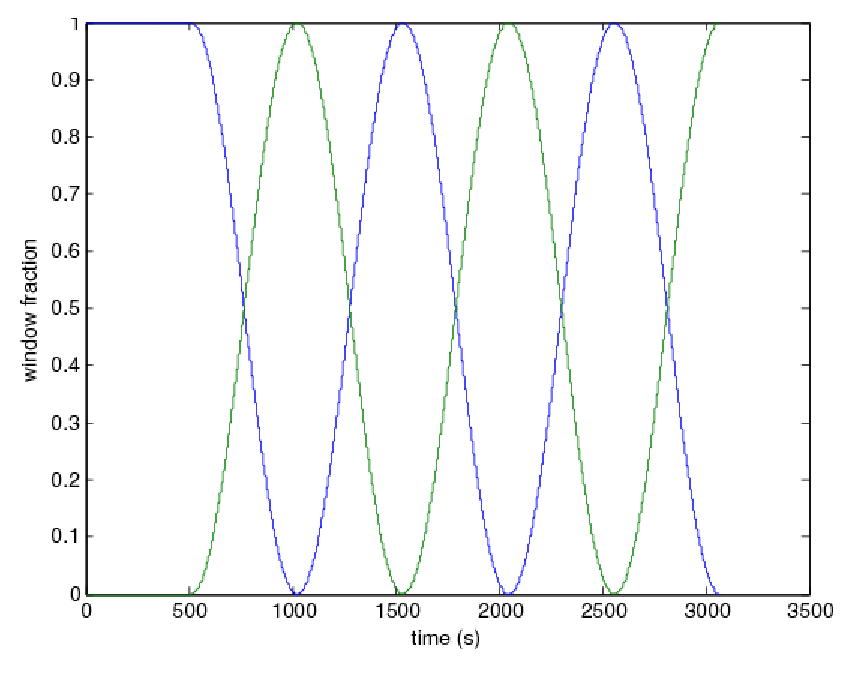
\includegraphics[height=95mm,width=120mm]{hann-windows.eps}
\caption{\textit{Windowing}}
\end{figure}
One job per science segment, filters are calculated for 1024 s windows;
50\%-overlapping Hann windows merged, AMPS h(t) frames written. Code in LIGO SVN:\\
\texttt{matapps/packages/detchar/}\\
\texttt{AMPS/trunk/eleutheria.m}
        Feedforward program structure: out-of-loop.

        \subsection{Data frame generation}
        \label{data_frames}
        
            Matlab: write frame files on cluster.

        \subsection{Post-processing diagnostics}
        \label{diagnostics}
 
LIGO Hanford h(t) spectrum after filtering MICH \& PRC:\\
noise floor in bucket falls quiet, freeing inspiral range.

\begin{figure}
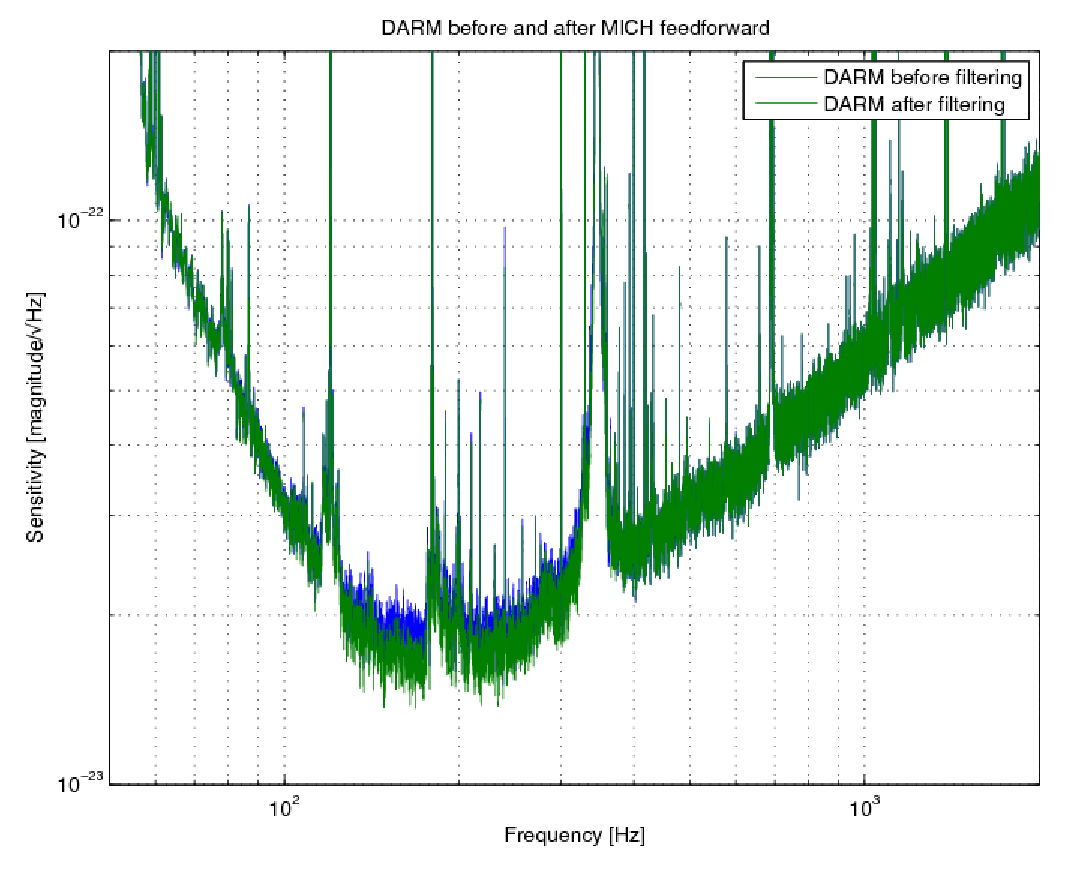
\includegraphics[height=80mm, width=60mm]{clip-exemplar-ASD.eps}
\caption{Exemplar, +1.1 Mpc (5.9\% inspiral range)
\textit{(GPS 953164819 to 953165839, 2010-03-21)}}
\end{figure}
\begin{figure}
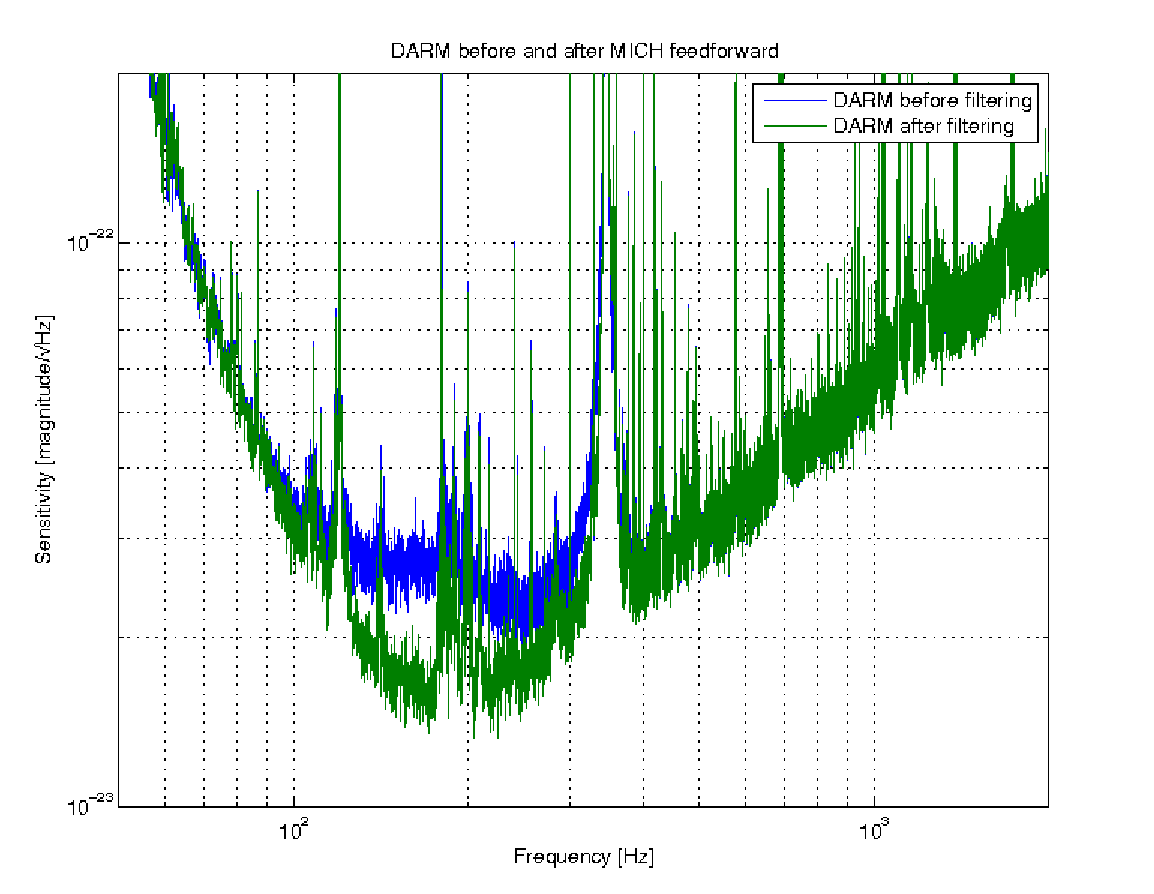
\includegraphics[height=80mm, width=60mm]{title_spectrum.eps}
\caption{Best seen, +4.4 Mpc (29\% inspiral range)
\textit{(GPS 955187679 to 955188191, 2010-04-13)}}
\end{figure}
\begin{figure}
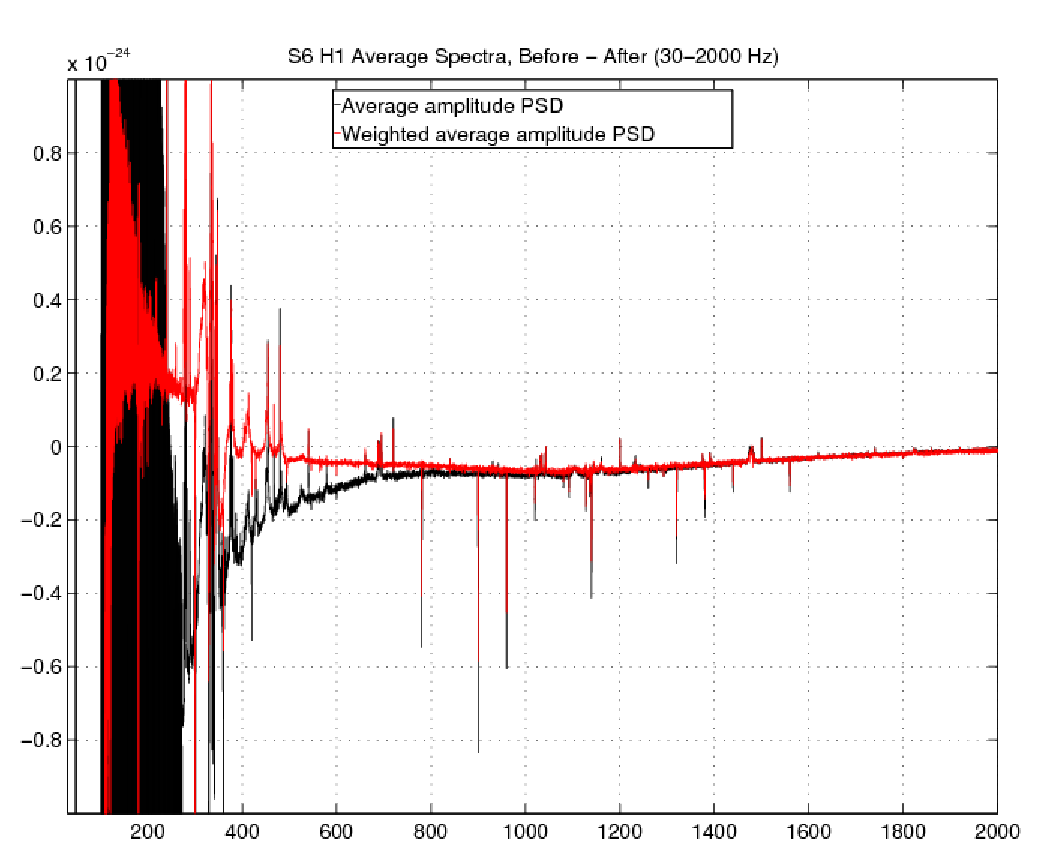
\includegraphics[height=80mm, width=60mm]{clip-diff.eps}
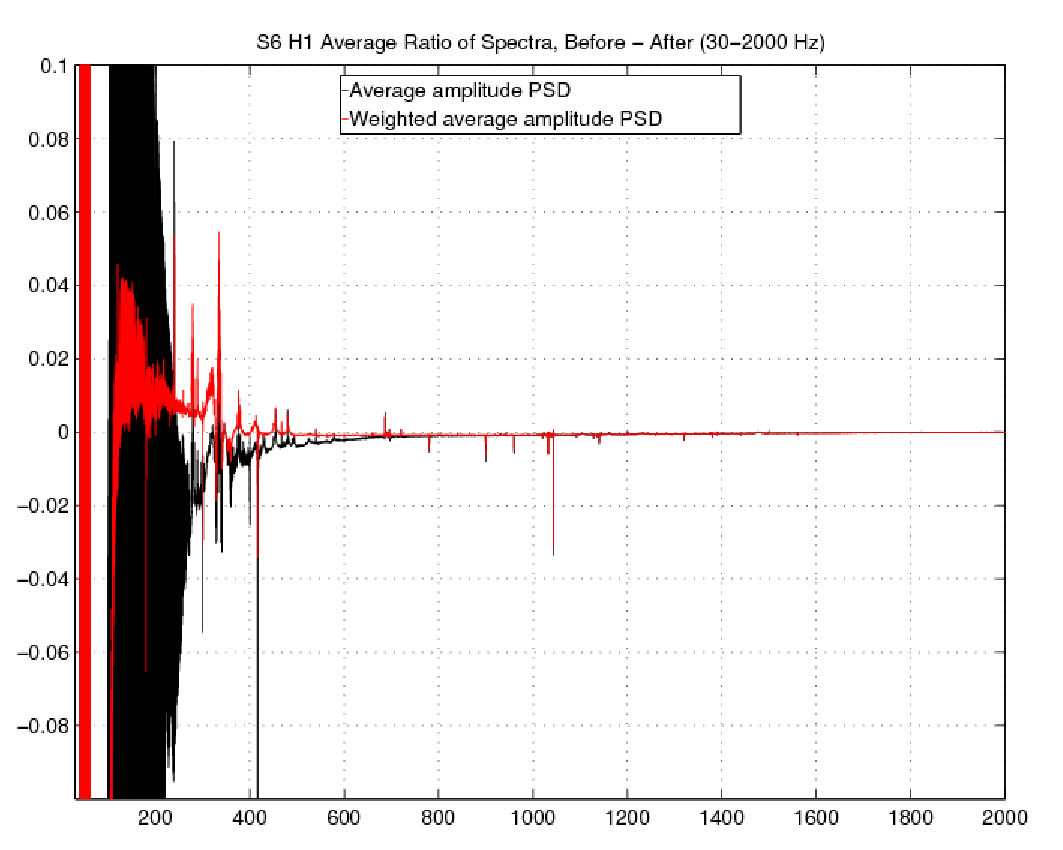
\includegraphics[height=80mm, width=60mm]{clip-diff-ratio.eps}
\caption{Arithmetic (black) \& harmonic (red) mean,
200 jobs: \textit{(before-after)} (L), \textit{(before-after)/before} (R)}
\end{figure}

            Matlab/Python/C: diagnostics -- combs, SFTs, range and data consistency.

            Many post-processing diagnostics, injections included. We tested the syncronization, before and after, with ringdown and sine-gaussian burst injections, and additionally we looked for any evidence of a frequency comb at the windowing frequency. No problems were found.

	    This is probably the optimal place to talk about the work that Ian Harry and maybe James Clark, David Keital and Karl Wette are doing, as well.

        \subsection{Feedforward benefits and potential}
        \label{benefits}

            Fine tuning, how data improves, potential for future.

Inspiral range, the distance at which coalescing neutron stars are likely to be detected, increases for both LIGO observatories when data from science run 6 is filtered. \textit{Post facto} feedforward noise subtraction improves performance.

\begin{figure}
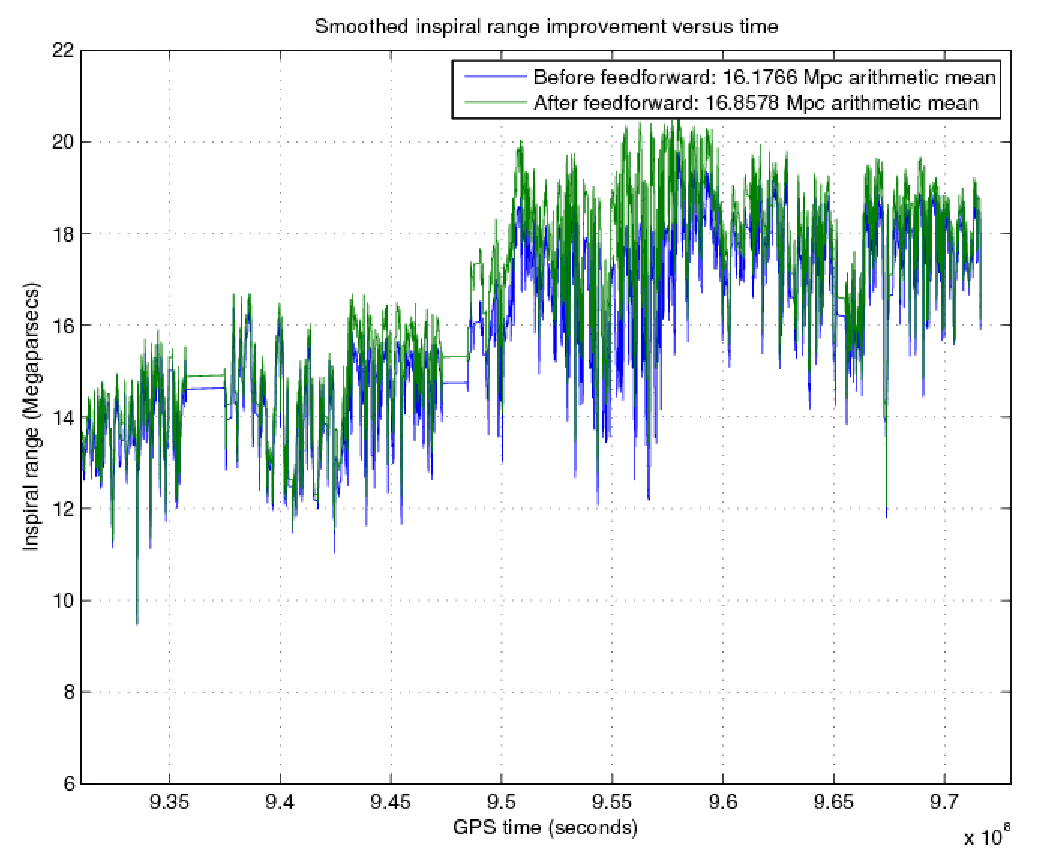
\includegraphics[height=60mm, width=120mm]{clip-range-LHO-new.eps}
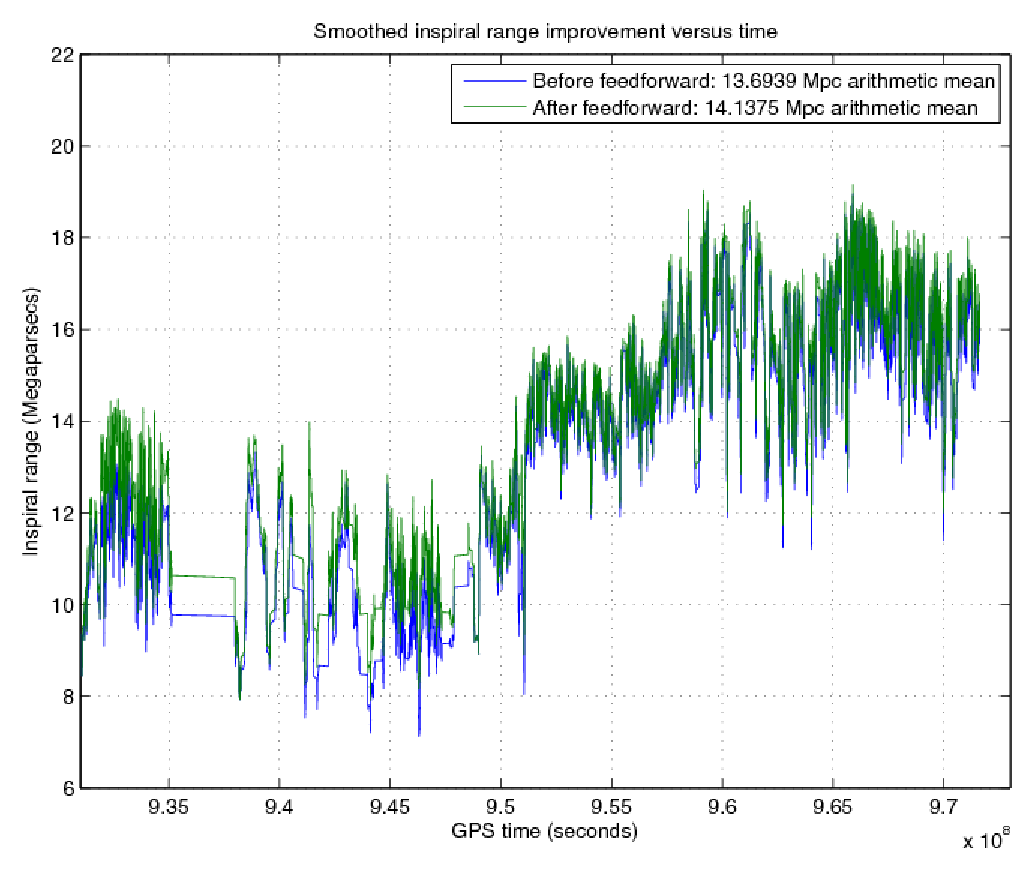
\includegraphics[height=60mm, width=120mm]{clip-range-LLO-new.eps}
\caption{Inspiral range vs time:
LHO (L) gains 0.69 Mpc, LLO (R) gains 0.43 Mpc}
\end{figure}
\begin{figure}
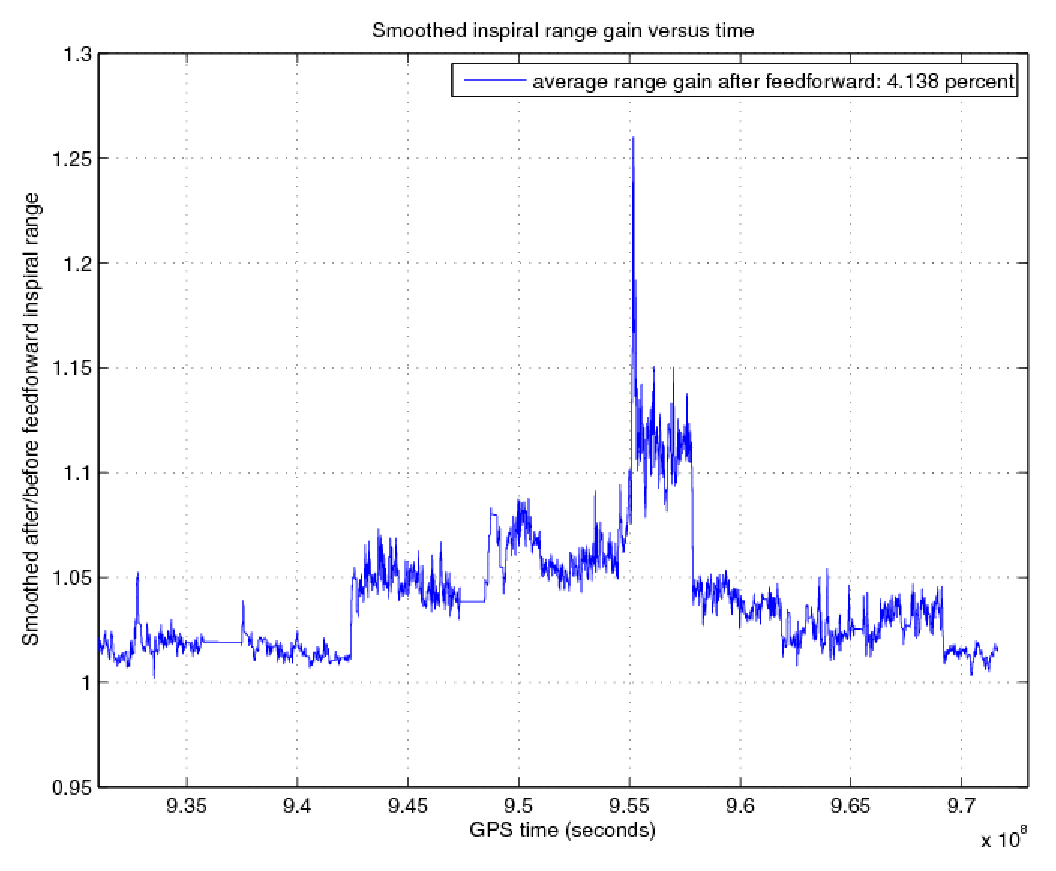
\includegraphics[height=60mm, width=120mm]{clip-gain-LHO-new.eps}
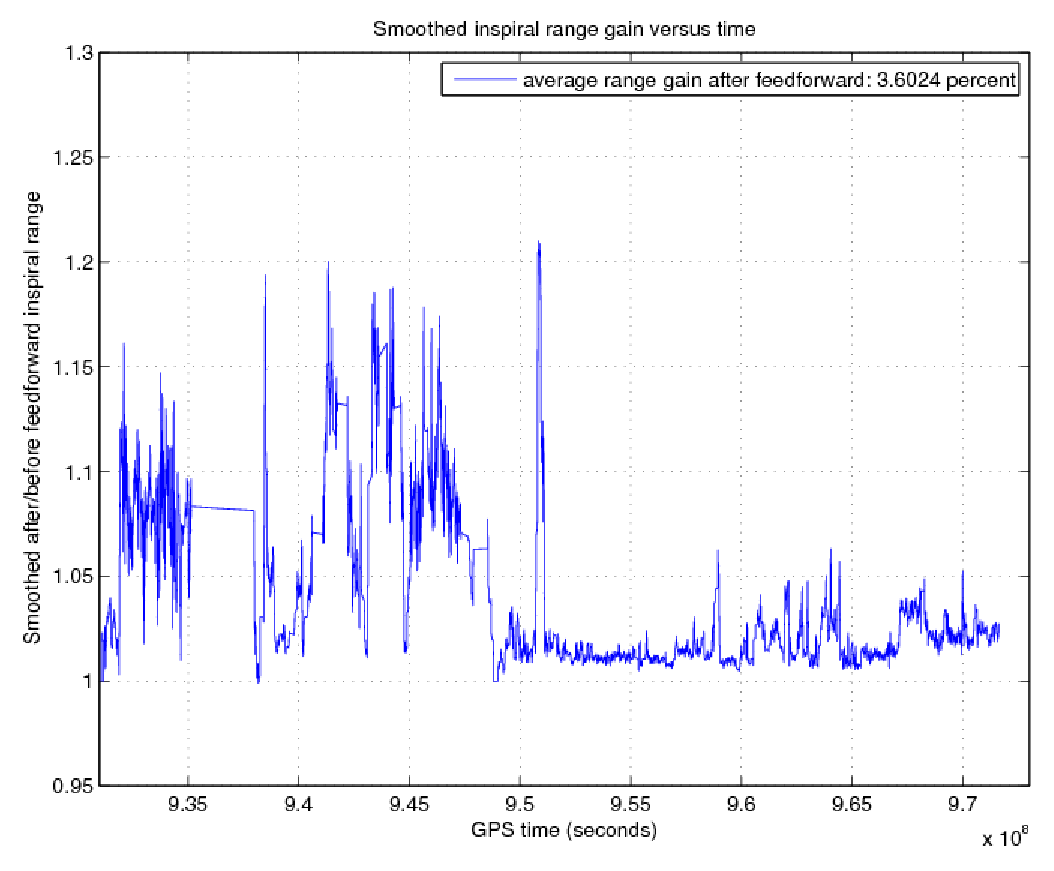
\includegraphics[height=60mm, width=120mm]{clip-gain-LLO-new.eps}
\caption{Inspiral range \textit{fractional gain} vs time:
LHO (L) 4.13\% better, LLO (R) 3.60\% better}
\end{figure}
\begin{figure}
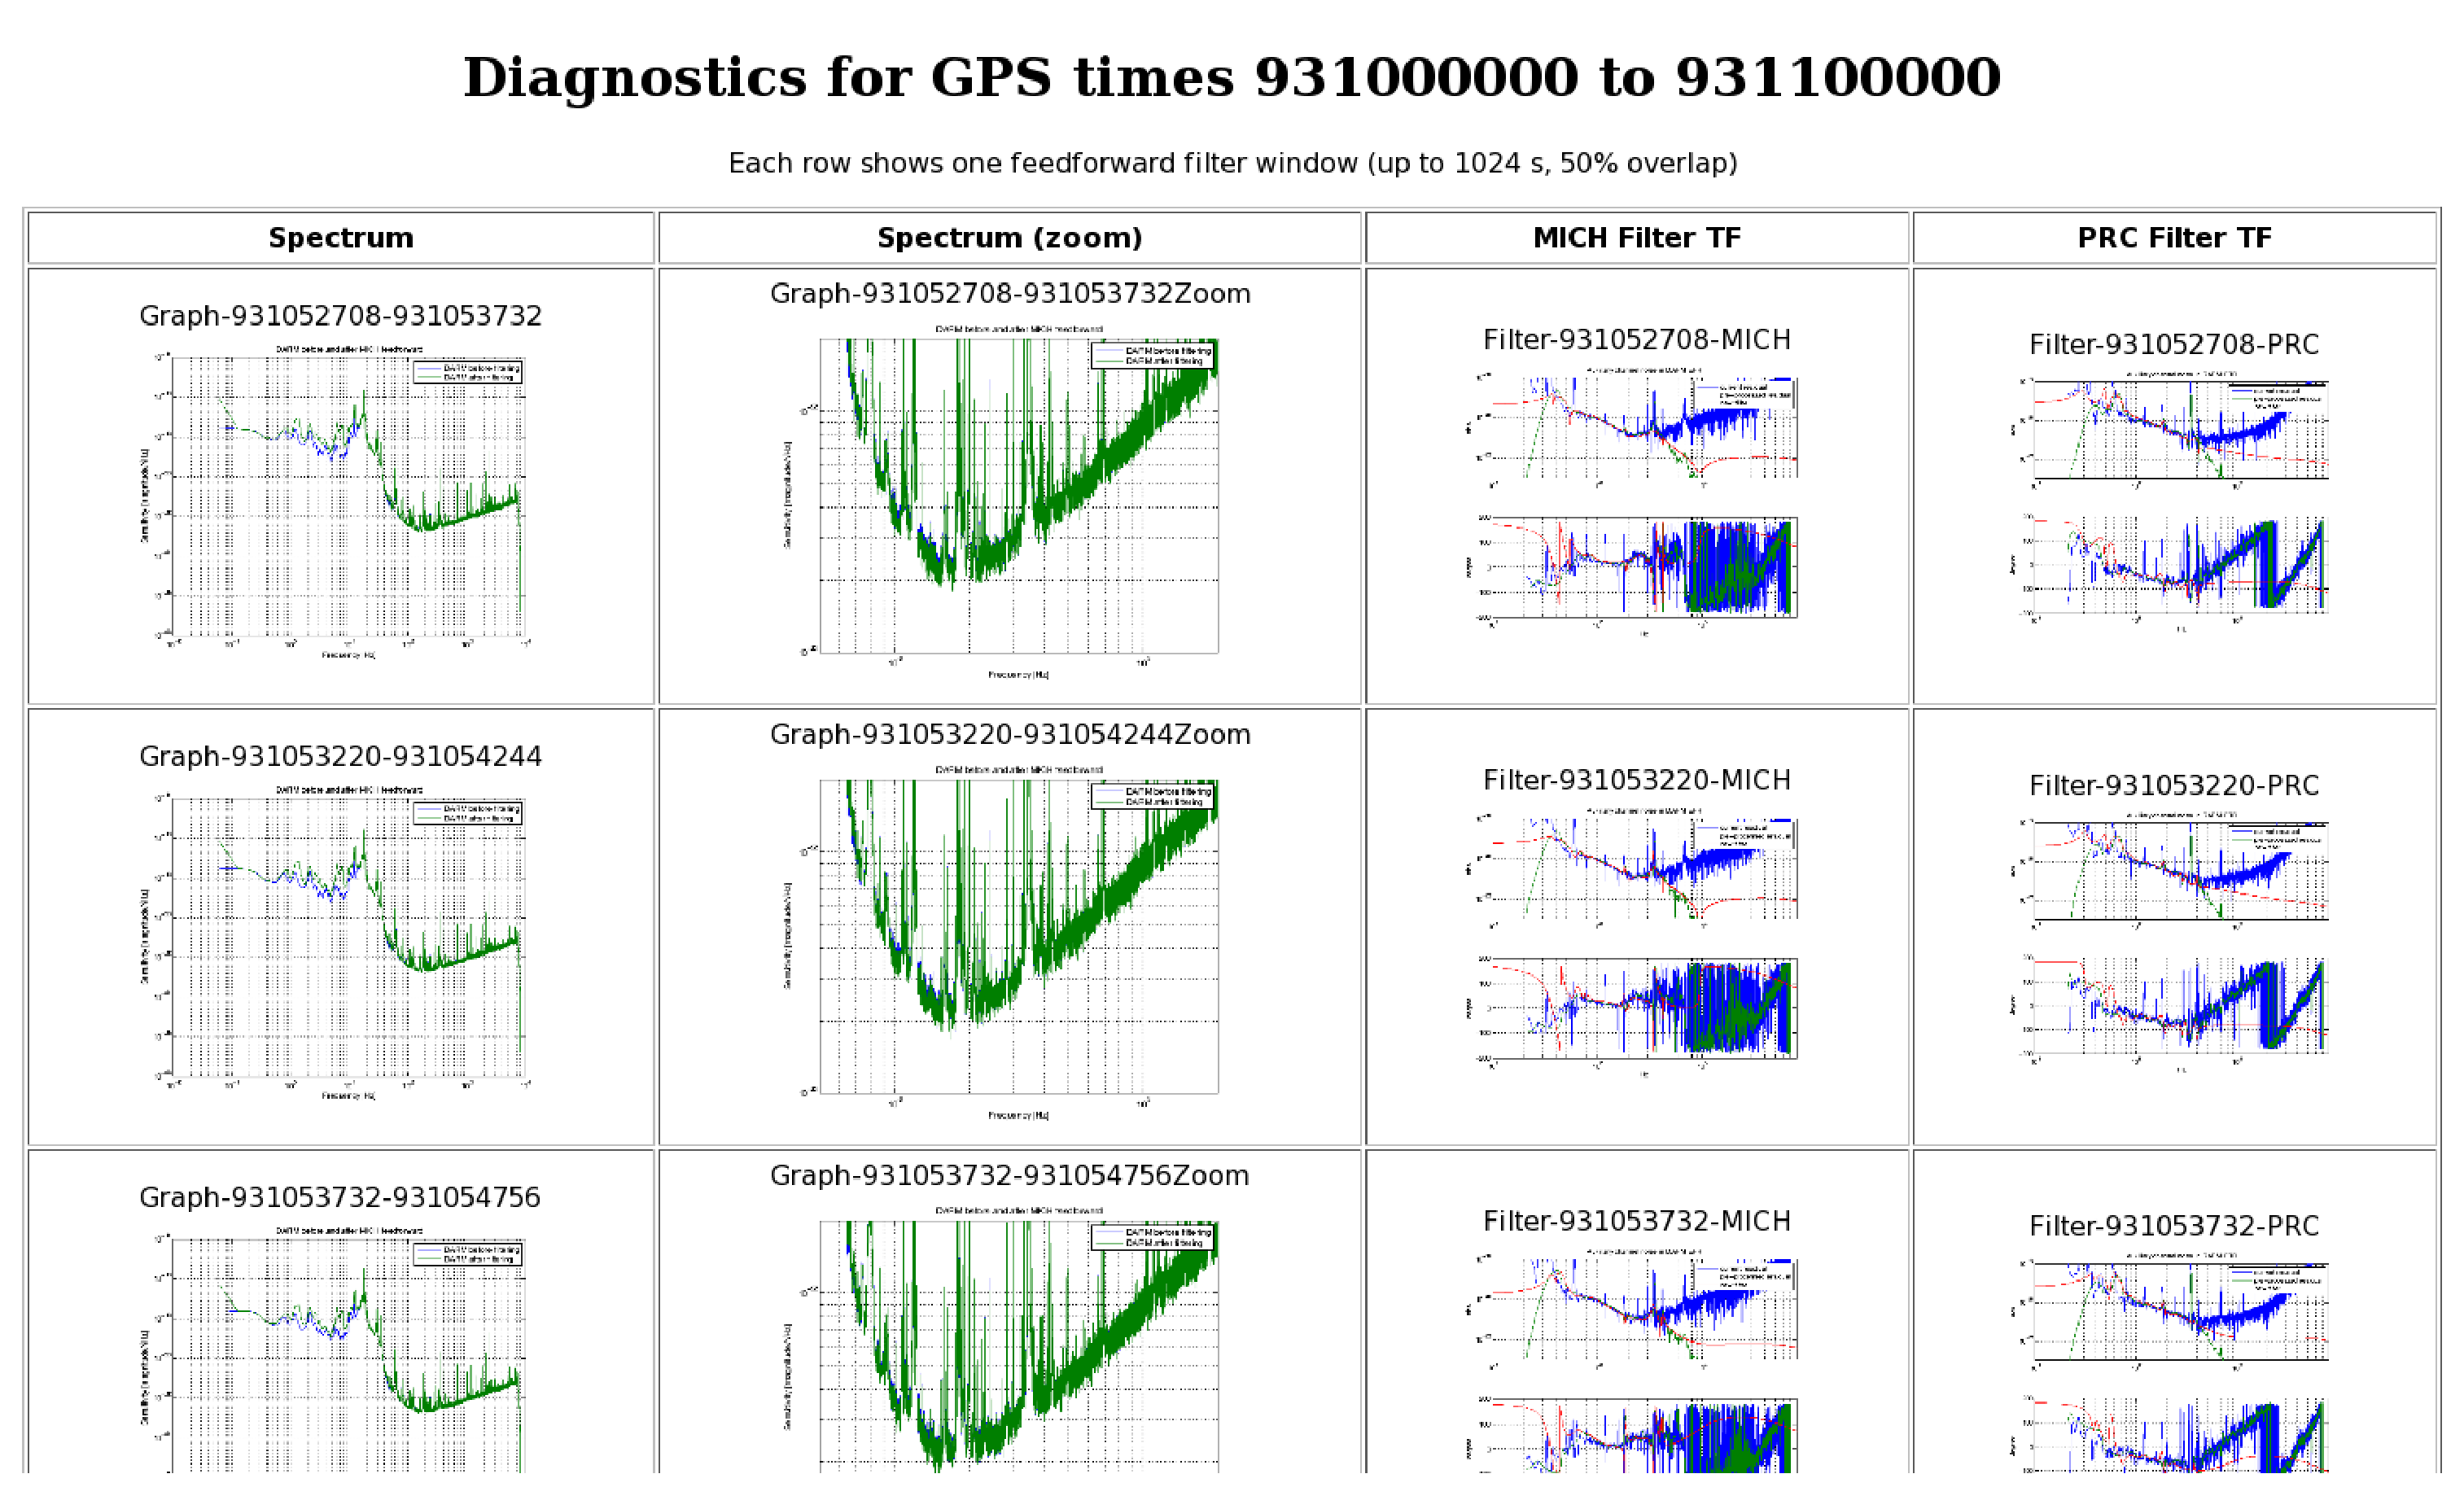
\includegraphics[height=60mm, width=120mm]{croppedWebpage.eps}
\caption{Webpages, window-by-window: \newline \texttt{https://ldas-jobs.ligo.caltech.edu/} \texttt{\~{}pulsar/feedforward/diagnostics}}
\end{figure}

\begin{itemize}
\item[1]. Feedforward subtracts noise using Vectfit to fit a transfer function between noise \& signal
\item[2]. h(t) is filtered with MICH \& PRC, range improves 4 \% (volume 12 \%), minimum strain about ten percent better.
\item[3]. AMPS frames for S6 LHO \& LLO exist at CIT:
\texttt{/archive/frames/S6/pulsar/feedforward}
\item[4]. The \textit{best} h(t) \& inspiral range of any site/time till Advanced LIGO is on these frames 
\item[5]. Advanced LIGO could use such methods to characterize MICH \& PRC changes, fix quickly, even \textit{post facto}
\end{itemize}
 
\textit{References}:
LIGO optical pathlength definitions via Adhikari~\cite{AdhikariThesis} and~\cite{BallmerThesis}; Vectfit developed by Gustavsen et al~\cite{Deschrijver2008},~\cite{Gustavsen2006},~\cite{Gustavsen1999}. Remember to note that Tobin Fricke wrote the function that applies the ZPKs as a SOS section-order-sections filter to the actual data, filterZPKs.m.

%        -----------------------------
%
%	The following is an example of using the commands \textit{ref}
%	and \textit{label}. With these commands theorems, chapters,
%	sections and figurres can be labeld with names in the tex file
%	and then refered to by these names in later tex files. In
%	chapter~\ref{intro} we saw section~\ref{sample_section} or
%	theorem~\ref{sample_theorem}.
%
%	Lastly, here is how to include a figure. First generate an
%	encapsulated postscript file in xfig, adobe illustrator or
%	some other program. The specific commands are found in
%	\textit{chap2.tex}.
%
%        \begin{figure}[htb]
%        \centerline{ \epsfig{figure=sample.eps, 
%        height =  1.5 in}}
%        \caption{Sample Figure}
%        \label{sample_figure}
%        \end{figure}

